\chapter{Outline}
\label{chap:out}

This thesis is divided into two parts. The first details my work on Bayesian inference, and the second in inflationary cosmology.
The first chapter of each part (Chapters~\ref{chap:cos} and~\ref{chap:bay}) are introductory, establishing basic theory and notation. The remainder of the thesis is entirely my own work, except where references explicitly state otherwise.

\section{The big picture}
\begin{figure}
  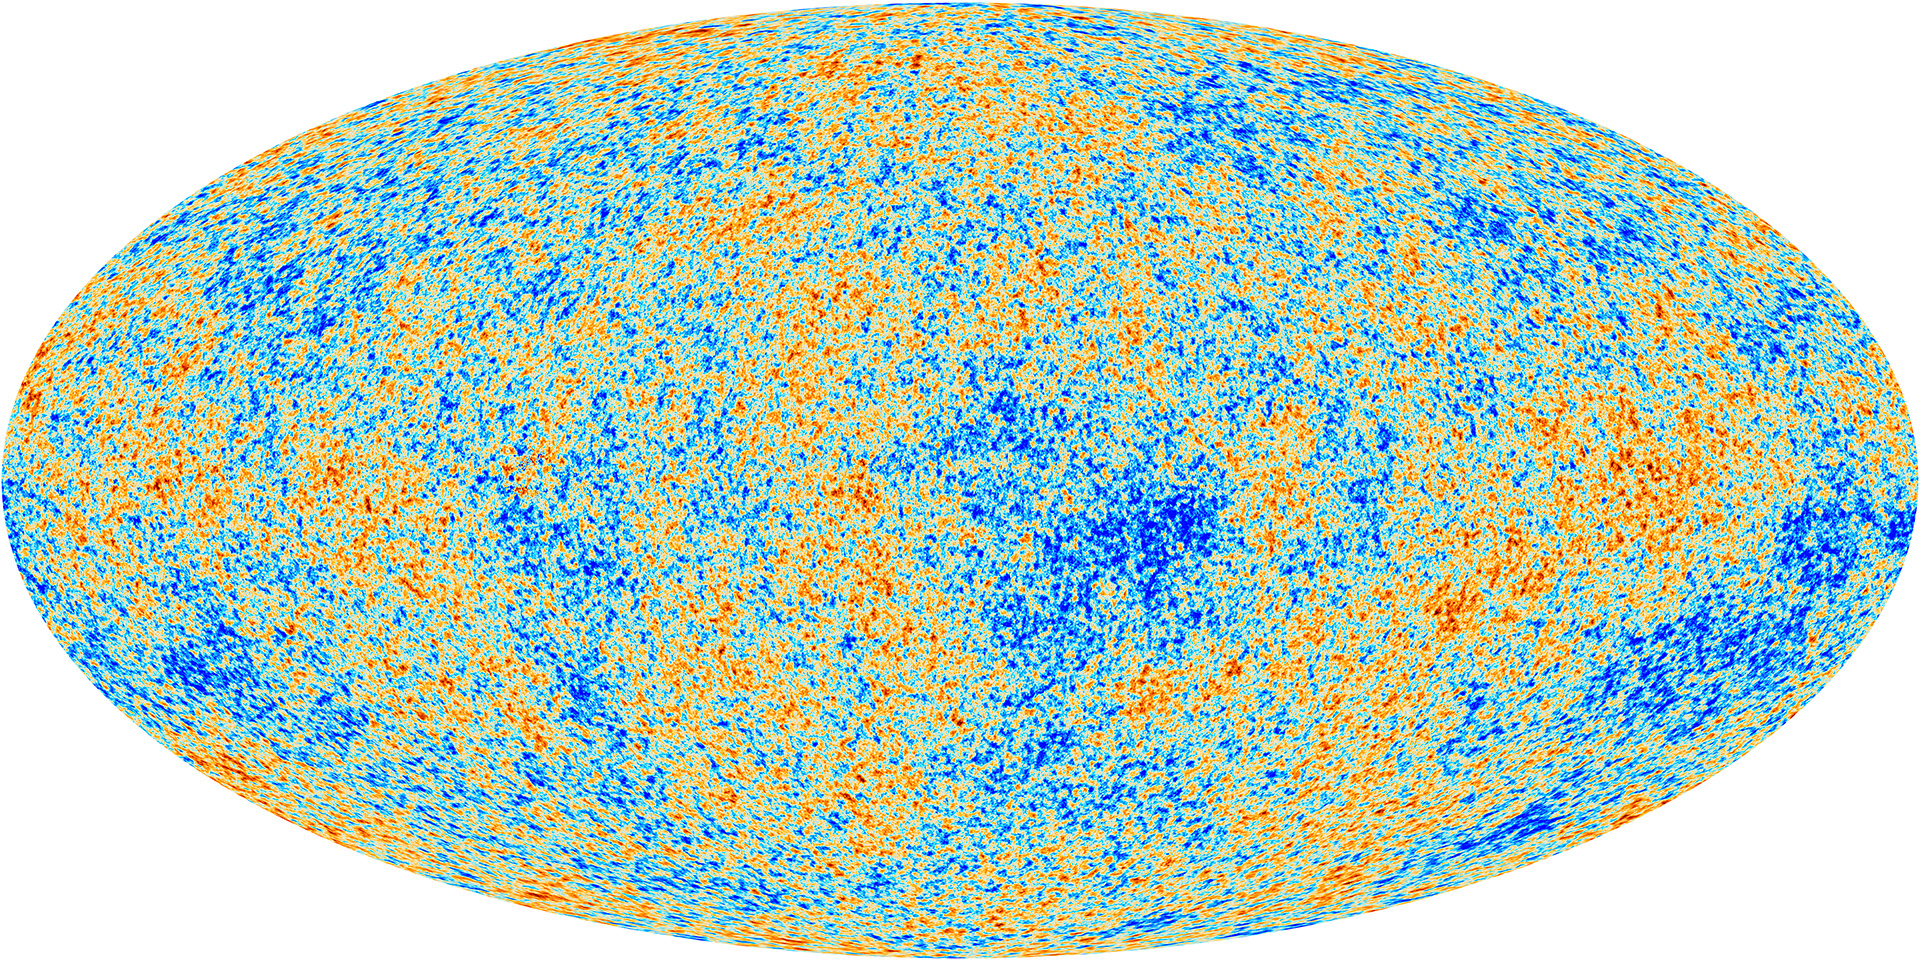
\includegraphics[width=\textwidth]{chapter_outline/figures/planck}
  \caption{Planck's image of the early universe}\label{fig:out:planck}
\end{figure}

As cosmologists, nature has been incredibly kind to us. We have been given a near crystal clear snapshot of the universe a mere 300,000 years after its birth. Images taken by the Planck satellite (Figure~\ref{fig:out:planck}) show the universe at this time, detailing the regions of higher and lower density. For cosmologists this is interesting in two ways. 

First, these distortions in density are the beginnings of the formation of stars, galaxies and galaxy clusters. If one were to wind the clock forwards from this moment we would see cosmic structure coalescing around the regions of higher density.

Second, these distortions tell us a great deal about physics at much earlier times. Observations from particle physics experiments allow us to confidently wind the clock backwards to mere microseconds after the big bang.
However, the expansion of the universe itself allows us to look even further back than this. We now have a wealth of evidence that early in its history, the universe went though a rapid accelerated epoch.  This expansion acts as a cosmic magnifying glass, allowing us to observe patterns $\sim10^{-32}$ seconds after the big bang using the universe we see today. The upshot of this is that cosmologists effectively have access the to most powerful particle accelerator imaginable, trillions of times stronger than the Large Hadron Collider. 

The canonical explanation for the early period of accelerated expansion is the theory of inflation, with quantum fields providing the necessary driving force. Part~\ref{part:cosmology} of this thesis focusses on the initial conditions for inflation; i.e.\ what started this all off.

\section{Kinetic initial conditions}

Traditionally, cosmologists work under the assumption that at these early times the universe was in an effectively beginningless inflating state, with no detectable beginning. Chapter~\ref{chap:kd} rigorously proves a result that suggests this picture was somewhat incomplete.  Instead, almost all classical universes begin at a finite time in the past.  Moreover this beginning is dominated by kinetic energy, and not inflating. This provides a novel and arguably simpler mechanism for setting the initial conditions of the universe. More importantly, I also show that this period could have produced a distinct observational signature in the primordial power spectrum of curvature perturbations.

Chapter~\ref{chap:rec} details a reconstruction of this primordial spectrum which was conducted as part of the Planck collaboration. Whilst not conclusive, it did show tantalising hints of a signal consistent with a pre-inflationary epoch.

\section{Observations in high dimensions}
\begin{figure}
  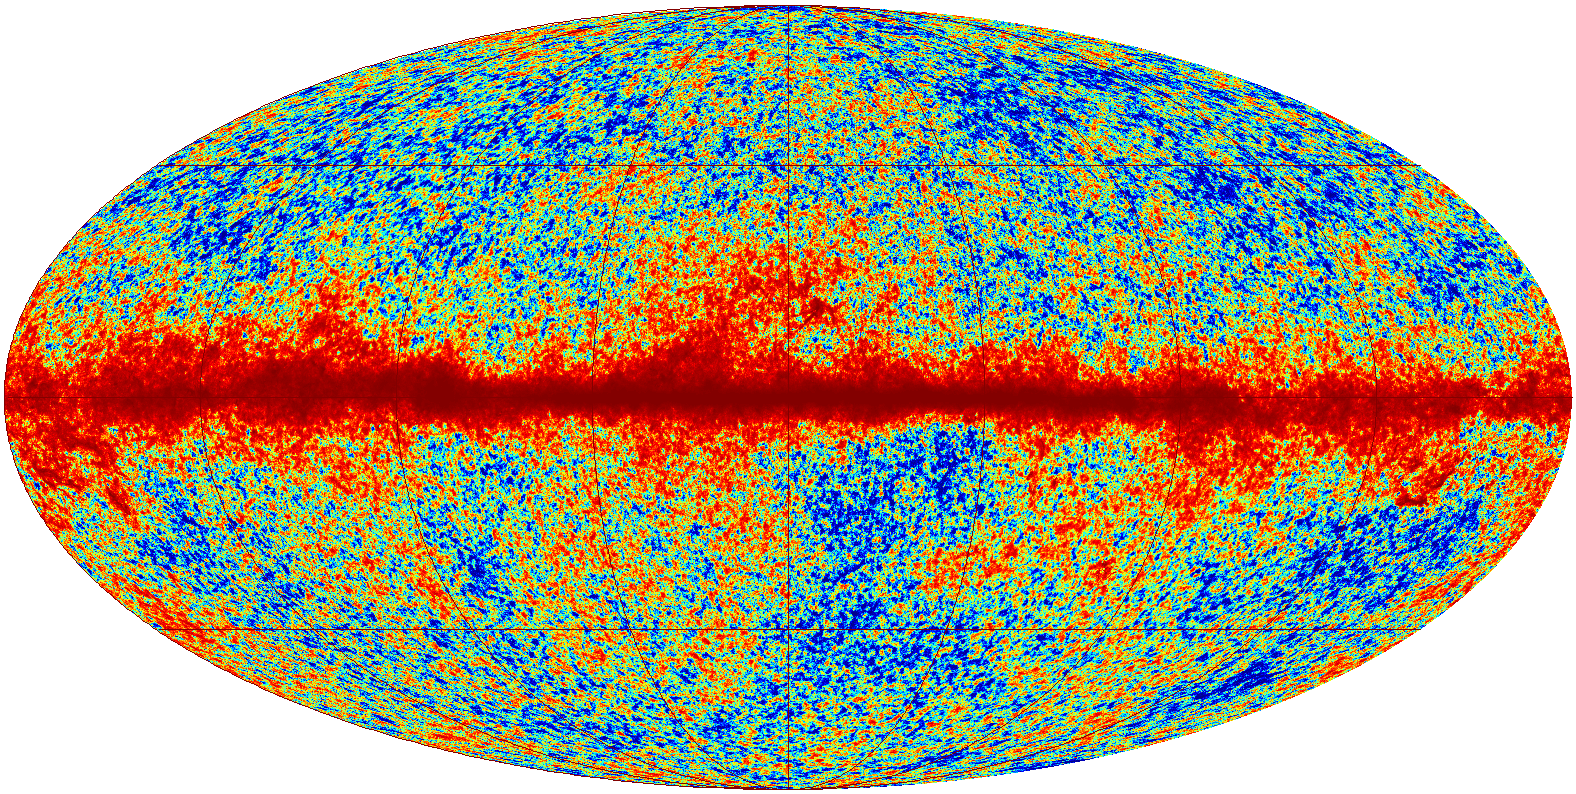
\includegraphics[width=\textwidth]{chapter_outline/figures/planck_galaxy}
  \caption{The actual image taken by Planck}\label{fig:out:planck_galaxy}
\end{figure}
Planck's view of the early universe is not in fact the one shown in Figure~\ref{fig:out:planck}. The picture it actually takes is more akin to Figure~\ref{fig:out:planck_galaxy} (Figure~\ref{fig:out:planck} in fact being a processed image). The obvious difference between the two is the presence of a red band in the center of the image, which are the microwaves emitted by our own Milky Way galaxy. In order to observe the microwaves from by the beginning of the universe, we must first remove the contaminating information of the Milky Way. This requires a sophisticated model of the galaxy, with many parameters that must be simultaneously determined and quantified. 

Whilst working on Planck, it became apparent that the principle difficulty of searching for this signal was an absence of data analysis tools. There was no servicable method for analysing complicated Bayesian models such as those found in the galactic foregrounds.

The Cavendish astrophysics department has long been a pioneer in proposing and developing groundbreaking Bayesian statistical approaches. With this in mind, I designed and implemented a novel algorithm which was christened PolyChord (detailed in Part~\ref{part:statistics} in Chapter~\ref{chap:pc}). This was designed to gather information from data about complicated scientific models, whilst simultaneously calculating the probability that the model is true. PolyChord proved extremely successful in the Planck analysis, and was rapidly adopted by many members of the team as its de Facto inference tool

\section{Quantum initial conditions}
My latest work focusses on the quantum mechanical initial conditions of the early universe. A full theoretical treatment of this epoch requires a consideration of quantum fields in curved spacetime, a discipline that was pioneered by our own Professor Hawking. One of the critical issues is that our basic ideas about how we talk about quantum particles are not designed to work in the context of gravity as a curved spacetime background. My latest research aims to resolve some of these issues, by re-defining the quantum mechanical notion of empty space. I also demonstrated that in the context of the early universe this alternative viewpoint makes detectable predictions which again differ from standard theory. This is detailed in Chapter~\ref{chap:qv}.

Whilst examining this, I realised that I needed a better way of solving the equations of the early universe. Whilst this is not central to my physics research, I did indeed succeeded in developing a novel class of extremely efficient numerical methods for solving these, which I term RKWKB approaches. RKWKB is explained in Part~\ref{part:statistics}, Chapter~\ref{chap:RK}.




